\documentclass[aspectratio=169,11pt]{beamer}

% ============================================================
% PACKAGES
% ============================================================
\usepackage{graphicx}
\usepackage{tikz}
\usetikzlibrary{positioning,arrows.meta}
\usepackage{xcolor}
\usepackage{booktabs}
\usepackage{tabularx}
\usepackage{array}
\usepackage{ragged2e}
\usepackage{hyperref}

% ============================================================
% COLORS - SAME AS PHASE-I
% ============================================================
\definecolor{GEUBlue}{RGB}{20,55,105}
\definecolor{GEULightBlue}{RGB}{238,244,251}
\definecolor{GEUGrey}{RGB}{90,90,90}
\definecolor{GEULightGrey}{RGB}{245,246,248}

% ============================================================
% BEAMER SETTINGS
% ============================================================
\usetheme{default}
\setbeamertemplate{navigation symbols}{}
\setbeamertemplate{blocks}[rounded][shadow=false]

\setbeamercolor{normal text}{fg=black,bg=white}
\setbeamercolor{frametitle}{fg=GEUBlue}
\setbeamercolor{structure}{fg=GEUBlue}
\setbeamercolor{block title}{fg=GEUBlue,bg=GEULightBlue}
\setbeamercolor{block body}{fg=black,bg=GEULightBlue}

\setbeamerfont{frametitle}{size=\Large,series=\bfseries}

% ============================================================
% LOGO
% ============================================================
% Upload Graphic Era logo as graphicera_logo.png
\newcommand{\GEULogo}{graphicera_logo.png}

% ============================================================
% HEADER
% ============================================================
\setbeamertemplate{headline}{%
  \begin{tikzpicture}[remember picture,overlay]
    \node[
        anchor=north east,
        xshift=-0.30cm,
        yshift=-0.12cm
    ] at (current page.north east)
    {\includegraphics[height=0.62cm]{\GEULogo}};
  \end{tikzpicture}
  \vspace{0.72cm}
}

% ============================================================
% FRAME TITLE
% ============================================================
\setbeamertemplate{frametitle}{%
  \vspace{0.03cm}
  \insertframetitle\par
  \vspace{0.04cm}
  \textcolor{GEUBlue}{\rule{\textwidth}{0.9pt}}
  \vspace{0.03cm}
}

% ============================================================
% FOOTER
% ============================================================
\setbeamertemplate{footline}{%
  \leavevmode
  \hbox{%
  \begin{beamercolorbox}[
      wd=.82\paperwidth,
      ht=0.32cm,
      dp=0.10cm,
      leftskip=.3cm
  ]{author in head/foot}
    \tiny Department of Computer Science \& Engineering |
    Graphic Era (Deemed to be University)
  \end{beamercolorbox}%
  \begin{beamercolorbox}[
      wd=.18\paperwidth,
      ht=0.32cm,
      dp=0.10cm,
      rightskip=.3cm
  ]{date in head/foot}
    \hfill\tiny\insertframenumber/\inserttotalframenumber
  \end{beamercolorbox}}
}

% ============================================================
% CUSTOM COMMANDS
% ============================================================
\newcommand{\smallnote}[1]{%
\vspace{0.08cm}
{\scriptsize\color{GEUGrey}#1}
}

\newcommand{\placeholder}[1]{%
\textit{\color{GEUGrey}#1}
}

% ============================================================
% DOCUMENT INFORMATION
% ============================================================
\title{\textbf{Project-Based Learning}\\[2mm]\large Phase-III Evaluation}

\author{
\textbf{Project Title}\\
Team ID: XXXX
}

\institute{
Department of Computer Science \& Engineering\\
Graphic Era (Deemed to be University), Dehradun
}

\date{Academic Session 2026--27}

% ============================================================
% DOCUMENT
% ============================================================
\begin{document}

% ============================================================
% SLIDE 1
% ============================================================
\begin{frame}[plain]

\begin{tikzpicture}[remember picture,overlay]

\draw[GEUBlue,line width=3pt]
(current page.north west) -- (current page.north east);

\node[
    anchor=north east,
    xshift=-0.45cm,
    yshift=-0.35cm
] at (current page.north east)
{\includegraphics[height=1.0cm]{\GEULogo}};

\node[
    align=center,
    text width=.84\paperwidth
] at ([yshift=.25cm]current page.center)
{
{\color{GEUBlue}
\fontsize{26}{30}\selectfont
\bfseries PROJECT-BASED LEARNING}
\\[3mm]

{\fontsize{18}{22}\selectfont
PHASE-III FINAL EVALUATION}
\\[7mm]

{\color{GEUGrey}
\Large\bfseries
\placeholder{Project Title}}
\\[3mm]

{\color{GEUBlue}
\normalsize Team ID: XXXX}
};

\node[
    align=center,
    anchor=south,
    yshift=.42cm
] at (current page.south)
{
\bfseries
Department of Computer Science \& Engineering\\
Graphic Era (Deemed to be University), Dehradun\\[-1mm]
\scriptsize Academic Session 2026--27
};

\end{tikzpicture}

\end{frame}

% ============================================================
% SLIDE 2
% ============================================================
\begin{frame}{Team \& Mentor Details}

\begin{columns}[T,totalwidth=\textwidth]

\column{.48\textwidth}

\begin{block}{Team Information}
\begin{tabular}{@{}ll@{}}
\textbf{Team ID:} & XXXX\\
\textbf{Semester:} & 3rd / 5th\\
\textbf{Section:} & XX\\
\textbf{Domain:} & \placeholder{XXXX}
\end{tabular}
\end{block}

\column{.48\textwidth}

\begin{block}{Team Members}
1.\quad \placeholder{Student Name -- ID}\\
2.\quad \placeholder{Student Name -- ID}\\
3.\quad \placeholder{Student Name -- ID}\\
4.\quad \placeholder{Student Name -- ID}
\end{block}

\end{columns}

\vspace{2mm}

\begin{block}{Mentor}
\placeholder{Dr. / Mr. / Ms. Mentor Name}
\hfill
\textbf{Interactions:} \underline{\hspace{12mm}}
\end{block}

\vfill

\smallnote{
Brief Discussion: Introduce the team, project domain and individual
technical responsibilities.
}

\end{frame}

% ============================================================
% SLIDE 3
% ============================================================
\begin{frame}{Project Abstract \& Problem Statement}

\begin{block}{Project Abstract}
\placeholder{
Provide a concise summary of the problem, proposed solution,
implementation and final outcome of the project.
}
\end{block}

\vspace{2mm}

\begin{block}{Problem Statement}
\placeholder{
Clearly state the real-world/technical problem addressed by the project.
}
\end{block}

\vspace{2mm}

\textbf{\color{GEUBlue}Target Users / Application}

\begin{itemize}\itemsep2pt
    \item \placeholder{Primary users / stakeholders}
    \item \placeholder{Application environment}
    \item \placeholder{Expected practical benefit}
\end{itemize}

\smallnote{
Brief Discussion: Explain the problem and final solution in a concise
manner without repeating the complete Phase-I presentation.
}

\end{frame}

% ============================================================
% SLIDE 4
% ============================================================
\begin{frame}{Objectives \& Final Deliverables}

\begin{columns}[T,totalwidth=\textwidth]

\column{.48\textwidth}

\textbf{\color{GEUBlue}Finalized Objectives}

\begin{enumerate}\itemsep3pt
    \item \placeholder{Objective 1}
    \item \placeholder{Objective 2}
    \item \placeholder{Objective 3}
    \item \placeholder{Objective 4}
    \item \placeholder{Objective 5}
\end{enumerate}

\column{.48\textwidth}

\textbf{\color{GEUBlue}Final Deliverables}

\begin{itemize}\itemsep3pt
    \item \placeholder{Working prototype/system}
    \item \placeholder{Source code}
    \item \placeholder{Database/dataset}
    \item \placeholder{Documentation}
    \item \placeholder{Other technical outcome}
\end{itemize}

\end{columns}

\vfill

\smallnote{
Brief Discussion: Relate each objective to a tangible final deliverable.
}

\end{frame}

% ============================================================
% SLIDE 5
% ============================================================
\begin{frame}{Phase-I \& Phase-II Feedback Incorporated}

\scriptsize

\begin{center}

\renewcommand{\arraystretch}{1.35}

\begin{tabularx}{.96\textwidth}
{@{}p{2.1cm}X X@{}}

\toprule
\textbf{Phase} &
\textbf{Feedback / Suggestion} &
\textbf{Action Taken}\\
\midrule

Phase-I &
\placeholder{Feedback received during Phase-I} &
\placeholder{Modification incorporated}\\

Phase-I &
\placeholder{Feedback received during Phase-I} &
\placeholder{Modification incorporated}\\

Phase-II &
\placeholder{Feedback received during Phase-II} &
\placeholder{Modification incorporated}\\

Phase-II &
\placeholder{Feedback received during Phase-II} &
\placeholder{Modification incorporated}\\

\bottomrule

\end{tabularx}

\end{center}

\vfill

\begin{block}{Final Improvement}
\placeholder{
Briefly explain how the project improved from the initial proposal
to the final implementation.
}
\end{block}

\smallnote{
Brief Discussion: Evaluators should be able to clearly identify
how earlier feedback has improved the final project.
}

\end{frame}

% ============================================================
% SLIDE 6
% ============================================================
\begin{frame}{Final System Architecture}

\begin{center}

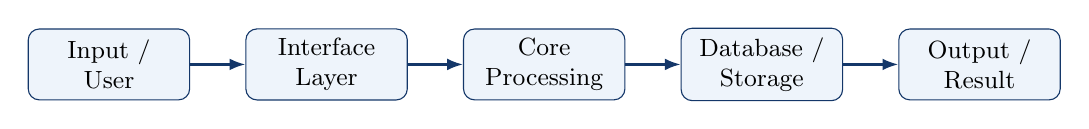
\begin{tikzpicture}[
node distance=7mm,
box/.style={
rectangle,
rounded corners,
draw=GEUBlue,
fill=GEULightBlue,
minimum width=2.05cm,
minimum height=9mm,
align=center,
font=\small
},
arrow/.style={
-{Latex[length=2mm]},
thick,
draw=GEUBlue
}
]

\node[box] (a) {Input /\\User};
\node[box,right=of a] (b) {Interface\\Layer};
\node[box,right=of b] (c) {Core\\Processing};
\node[box,right=of c] (d) {Database /\\Storage};
\node[box,right=of d] (e) {Output /\\Result};

\draw[arrow] (a)--(b);
\draw[arrow] (b)--(c);
\draw[arrow] (c)--(d);
\draw[arrow] (d)--(e);

\end{tikzpicture}

\end{center}

\vspace{4mm}

\begin{columns}[T,totalwidth=\textwidth]

\column{.48\textwidth}

\textbf{\color{GEUBlue}Major Components}

\begin{itemize}\itemsep2pt
    \item \placeholder{Component 1}
    \item \placeholder{Component 2}
    \item \placeholder{Component 3}
    \item \placeholder{Component 4}
\end{itemize}

\column{.48\textwidth}

\textbf{\color{GEUBlue}System Flow}

\begin{itemize}\itemsep2pt
    \item \placeholder{Input mechanism}
    \item \placeholder{Processing mechanism}
    \item \placeholder{Storage mechanism}
    \item \placeholder{Output mechanism}
\end{itemize}

\end{columns}

\vfill

\smallnote{
Brief Discussion: Replace the sample diagram with the actual final
architecture of the implemented system.
}

\end{frame}

% ============================================================
% SLIDE 7
% ============================================================
\begin{frame}{Final Technology Stack}

\begin{columns}[T,totalwidth=\textwidth]

\column{.48\textwidth}

\begin{block}{Software / Technologies}
\begin{itemize}\itemsep2pt
    \item Programming: \placeholder{XXXX}
    \item Framework: \placeholder{XXXX}
    \item Database: \placeholder{XXXX}
    \item Libraries/APIs: \placeholder{XXXX}
    \item OS/Platform: \placeholder{XXXX}
\end{itemize}
\end{block}

\column{.48\textwidth}

\begin{block}{Development Infrastructure}
\begin{itemize}\itemsep2pt
    \item IDE: \placeholder{XXXX}
    \item Version Control: Git/GitHub
    \item Testing Tools: \placeholder{XXXX}
    \item Deployment: \placeholder{XXXX}
    \item Other Tools: \placeholder{XXXX}
\end{itemize}
\end{block}

\end{columns}

\vfill

\smallnote{
Brief Discussion: Justify the final technology choices and mention
any changes made from the initially proposed technology stack.
}

\end{frame}

% ============================================================
% SLIDE 8
% ============================================================
\begin{frame}{Implementation of PBL Course Concepts}

\scriptsize

\begin{center}

\renewcommand{\arraystretch}{1.25}

\begin{tabularx}{.96\textwidth}
{@{}>{\bfseries}p{2.8cm}X p{2.8cm}@{}}

\toprule
Course & Concepts Actually Implemented & Project Module\\
\midrule

Data Structures in C &
\placeholder{Arrays, Lists, Trees, Graphs, Hashing, etc.} &
\placeholder{Module / Feature}\\

OOPs with C++ &
\placeholder{Classes, Inheritance, Polymorphism, STL, etc.} &
\placeholder{Module / Feature}\\

\midrule

Operating Systems &
\placeholder{Processes, Threads, IPC, Memory, Synchronization, etc.} &
\placeholder{Module / Feature}\\

DBMS &
\placeholder{SQL, Transactions, Indexing, Normalization, etc.} &
\placeholder{Module / Feature}\\

\bottomrule

\end{tabularx}

\end{center}

\vfill

\begin{center}
\colorbox{GEULightBlue}{
\parbox{.88\textwidth}{
\centering
\textbf{Requirement:}
Mention only concepts that are \textbf{actually implemented}
and can be demonstrated/explained during evaluation.
}}
\end{center}

\smallnote{
For 3rd Semester: Data Structures + OOPs with C++.
For 5th Semester: Operating Systems + DBMS.
}

\end{frame}

% ============================================================
% SLIDE 9
% ============================================================
\begin{frame}{Module-Wise Final Implementation}

\scriptsize

\begin{center}

\renewcommand{\arraystretch}{1.35}

\begin{tabularx}{.96\textwidth}
{@{}p{2.4cm}X p{2.0cm}p{2.0cm}@{}}

\toprule
\textbf{Module} &
\textbf{Implementation} &
\textbf{Responsible} &
\textbf{Status}\\
\midrule

\placeholder{Module 1} &
\placeholder{Major functionality implemented} &
\placeholder{Member} &
Completed\\

\placeholder{Module 2} &
\placeholder{Major functionality implemented} &
\placeholder{Member} &
Completed\\

\placeholder{Module 3} &
\placeholder{Major functionality implemented} &
\placeholder{Member} &
Completed\\

\placeholder{Module 4} &
\placeholder{Major functionality implemented} &
\placeholder{Member} &
Completed\\

\bottomrule

\end{tabularx}

\end{center}

\vspace{4mm}

\begin{center}
\colorbox{GEULightBlue}{
\parbox{.65\textwidth}{
\centering
\textbf{Final Project Completion:}
\placeholder{XX\%}
}}
\end{center}

\vfill

\smallnote{
Brief Discussion: Explain actual implementation rather than planned
features. Clearly identify any incomplete functionality.
}

\end{frame}

% ============================================================
% SLIDE 10
% ============================================================
\begin{frame}{Working System / Prototype Demonstration}

\begin{columns}[T,totalwidth=\textwidth]

\column{.43\textwidth}

\textbf{\color{GEUBlue}Major Working Features}

\begin{itemize}\itemsep3pt
    \item \placeholder{Feature 1}
    \item \placeholder{Feature 2}
    \item \placeholder{Feature 3}
    \item \placeholder{Feature 4}
    \item \placeholder{Feature 5}
\end{itemize}

\column{.53\textwidth}

\begin{block}{System Screenshot / Output}

\centering
\vspace{11mm}

\placeholder{
Insert screenshot of final working system
}

\vspace{11mm}

\end{block}

\end{columns}

\vfill

\smallnote{
Brief Discussion: A live demonstration of the working project should
be provided wherever applicable. PPT screenshots should support,
not replace, the actual demonstration.
}

\end{frame}

% ============================================================
% SLIDE 11
% ============================================================
\begin{frame}{Data / Database / Backend Implementation}

\begin{columns}[T,totalwidth=\textwidth]

\column{.48\textwidth}

\textbf{\color{GEUBlue}Data / Database}

\begin{itemize}\itemsep3pt
    \item \placeholder{Database / data source}
    \item \placeholder{Schema / data structure}
    \item \placeholder{Important tables / entities}
    \item \placeholder{Storage / retrieval method}
    \item \placeholder{Data validation}
\end{itemize}

\column{.48\textwidth}

\textbf{\color{GEUBlue}Backend / Core Logic}

\begin{itemize}\itemsep3pt
    \item \placeholder{Core processing}
    \item \placeholder{API / service}
    \item \placeholder{Algorithm / logic}
    \item \placeholder{Authentication / security}
    \item \placeholder{Error handling}
\end{itemize}

\end{columns}

\vfill

\smallnote{
Brief Discussion: Explain the actual internal working of the system.
Use schema, class, sequence, or data-flow diagrams wherever relevant.
}

\end{frame}

% ============================================================
% SLIDE 12
% ============================================================
\begin{frame}{Testing \& Validation}

\scriptsize

\begin{center}

\renewcommand{\arraystretch}{1.35}

\begin{tabularx}{.96\textwidth}
{@{}p{2.0cm}X X p{1.4cm}@{}}

\toprule
Test Type &
Expected Result &
Observed Result &
Status\\
\midrule

\placeholder{Unit Test} &
\placeholder{Expected result} &
\placeholder{Observed result} &
Pass\\

\placeholder{Integration} &
\placeholder{Expected result} &
\placeholder{Observed result} &
Pass\\

\placeholder{System Test} &
\placeholder{Expected result} &
\placeholder{Observed result} &
Pass\\

\placeholder{Other Test} &
\placeholder{Expected result} &
\placeholder{Observed result} &
\placeholder{Status}\\

\bottomrule

\end{tabularx}

\end{center}

\vspace{3mm}

\begin{block}{Validation Summary}
\placeholder{
Explain how the final system was tested and validated against
the project objectives and requirements.
}
\end{block}

\smallnote{
Brief Discussion: Testing claims should be supported by actual
test cases, logs, screenshots, measurements or experimental evidence.
}

\end{frame}

% ============================================================
% SLIDE 13
% ============================================================
\begin{frame}{Results \& Performance Analysis}

\begin{columns}[T,totalwidth=\textwidth]

\column{.48\textwidth}

\textbf{\color{GEUBlue}Key Results}

\begin{itemize}\itemsep3pt
    \item \placeholder{Metric / Result 1}
    \item \placeholder{Metric / Result 2}
    \item \placeholder{Metric / Result 3}
    \item \placeholder{Metric / Result 4}
\end{itemize}

\column{.48\textwidth}

\begin{block}{Graph / Result Evidence}

\centering
\vspace{10mm}

\placeholder{
Insert graph / chart / result screenshot
}

\vspace{10mm}

\end{block}

\end{columns}

\vfill

\smallnote{
Brief Discussion: Use measurable results wherever applicable.
Explain what the results mean rather than only displaying values.
}

\end{frame}

% ============================================================
% SLIDE 14
% ============================================================
\begin{frame}{GitHub Repository \& Development Evidence}

\begin{columns}[T,totalwidth=\textwidth]

\column{.45\textwidth}

\textbf{\color{GEUBlue}Repository Details}

\begin{itemize}\itemsep3pt
    \item Repository: \placeholder{GitHub URL}
    \item Branch: \placeholder{main / other}
    \item README.md: \placeholder{Updated}
    \item Contributors: \placeholder{All members}
    \item Documentation: \placeholder{Available}
\end{itemize}

\column{.51\textwidth}

\textbf{\color{GEUBlue}Development Evidence}

\begin{itemize}\itemsep3pt
    \item \placeholder{Regular commits}
    \item \placeholder{Meaningful commit messages}
    \item \placeholder{Individual commits}
    \item \placeholder{Latest source code}
    \item \placeholder{Complete commit history}
\end{itemize}

\end{columns}

\vfill

\begin{center}
\colorbox{GEULightBlue}{
\parbox{.88\textwidth}{
\centering
\textbf{Requirement:}
All members must be contributors and individual development
activity should be visible through the GitHub history.
}}
\end{center}

\end{frame}

% ============================================================
% SLIDE 15
% ============================================================
\begin{frame}{Individual Contribution}

\scriptsize

\begin{center}

\renewcommand{\arraystretch}{1.35}

\begin{tabularx}{.96\textwidth}
{@{}p{1.8cm}p{1.8cm}X p{1.5cm}@{}}

\toprule
Member &
Role &
Final Technical Contribution &
Commits\\
\midrule

\placeholder{Member 1} &
\placeholder{Role} &
\placeholder{Specific technical contribution} &
\placeholder{XX}\\

\placeholder{Member 2} &
\placeholder{Role} &
\placeholder{Specific technical contribution} &
\placeholder{XX}\\

\placeholder{Member 3} &
\placeholder{Role} &
\placeholder{Specific technical contribution} &
\placeholder{XX}\\

\placeholder{Member 4} &
\placeholder{Role} &
\placeholder{Specific technical contribution} &
\placeholder{XX}\\

\bottomrule

\end{tabularx}

\end{center}

\vspace{3mm}

\begin{block}{Individual Evaluation}
Every member must be able to explain, demonstrate and defend
their individual technical contribution.
\end{block}

\smallnote{
Brief Discussion: Contributions should be specific and verifiable
through implementation, GitHub activity and individual viva.
}

\end{frame}

% ============================================================
% SLIDE 16
% ============================================================
\begin{frame}{Challenges, Limitations \& Lessons Learned}

\begin{columns}[T,totalwidth=\textwidth]

\column{.48\textwidth}

\textbf{\color{GEUBlue}Challenges \& Solutions}

\begin{itemize}\itemsep3pt
    \item \placeholder{Challenge 1 -- Solution}
    \item \placeholder{Challenge 2 -- Solution}
    \item \placeholder{Challenge 3 -- Solution}
\end{itemize}

\vspace{2mm}

\textbf{\color{GEUBlue}Current Limitations}

\begin{itemize}\itemsep2pt
    \item \placeholder{Limitation 1}
    \item \placeholder{Limitation 2}
\end{itemize}

\column{.48\textwidth}

\textbf{\color{GEUBlue}Technical Learning}

\begin{itemize}\itemsep3pt
    \item \placeholder{Learning 1}
    \item \placeholder{Learning 2}
    \item \placeholder{Learning 3}
\end{itemize}

\vspace{2mm}

\textbf{\color{GEUBlue}Team Learning}

\begin{itemize}\itemsep2pt
    \item \placeholder{Collaboration / development learning}
    \item \placeholder{Problem-solving experience}
\end{itemize}

\end{columns}

\vfill

\smallnote{
Brief Discussion: Discuss genuine technical limitations and lessons
learned rather than presenting the project as having no limitations.
}

\end{frame}

% ============================================================
% SLIDE 17
% ============================================================
\begin{frame}{Final Outcomes, Applications \& Future Scope}

\begin{columns}[T,totalwidth=\textwidth]

\column{.32\textwidth}

\textbf{\color{GEUBlue}Final Outcomes}

\begin{itemize}\itemsep3pt
    \item \placeholder{Outcome 1}
    \item \placeholder{Outcome 2}
    \item \placeholder{Outcome 3}
\end{itemize}

\column{.32\textwidth}

\textbf{\color{GEUBlue}Applications}

\begin{itemize}\itemsep3pt
    \item \placeholder{Application 1}
    \item \placeholder{Application 2}
    \item \placeholder{Application 3}
\end{itemize}

\column{.32\textwidth}

\textbf{\color{GEUBlue}Future Scope}

\begin{itemize}\itemsep3pt
    \item \placeholder{Enhancement 1}
    \item \placeholder{Enhancement 2}
    \item \placeholder{Enhancement 3}
\end{itemize}

\end{columns}

\vspace{5mm}

\begin{block}{Tangible Project Outcome}
\placeholder{
Mention whether the project resulted in a working prototype,
deployment, dataset, research work, technical solution or other
demonstrable outcome.
}
\end{block}

\end{frame}

% ============================================================
% SLIDE 18
% ============================================================
\begin{frame}{References \& Project Resources}

\begin{columns}[T,totalwidth=\textwidth]

\column{.53\textwidth}

\textbf{\color{GEUBlue}References}

\begin{enumerate}\itemsep3pt
    \item \placeholder{Research paper / journal}
    \item \placeholder{Conference paper}
    \item \placeholder{Book / standard}
    \item \placeholder{Official documentation}
    \item \placeholder{Dataset / technical resource}
\end{enumerate}

\column{.43\textwidth}

\textbf{\color{GEUBlue}Project Resources}

\begin{itemize}\itemsep3pt
    \item GitHub: \placeholder{URL}
    \item Demo: \placeholder{URL / NA}
    \item Dataset: \placeholder{URL / NA}
    \item Documentation: \placeholder{URL / NA}
\end{itemize}

\vfill

\begin{center}

\colorbox{GEUBlue}{
\parbox{.82\textwidth}{
\centering
\color{white}
\Large\textbf{Thank You}\\[1mm]
\normalsize Questions \& Discussion
}}

\end{center}

\end{columns}

\end{frame}

\end{document}